\documentclass[11pt,a4paper]{article}

% Essential packages
\usepackage[utf8]{inputenc}
\usepackage[T1]{fontenc}
\usepackage{amsmath,amssymb,amsthm}
\usepackage{mathtools}
\usepackage{algorithm}
\usepackage{algpseudocode}
\usepackage{hyperref}
\usepackage{cleveref}
\usepackage{enumitem}
\usepackage{tikz}
\usetikzlibrary{trees,arrows.meta,positioning,shapes,arrows,calc,decorations.pathreplacing}
\usepackage{tcolorbox}
\usepackage{xcolor}
\usepackage{listings}
% Page geometry
\usepackage[margin=1in]{geometry}

% Custom colors
\definecolor{darkblue}{RGB}{0,0,139}
\definecolor{darkgreen}{RGB}{0,100,0}
\definecolor{darkred}{RGB}{139,0,0}

% Custom box for key concepts
\newtcolorbox{keypoint}{colback=blue!5!white,colframe=blue!75!black,title=Key Point}
\newtcolorbox{highlight}{colback=yellow!10!white,colframe=orange!75!black}

% Better spacing in equations
\setlength{\jot}{10pt}

% Theorem environments
\theoremstyle{plain}
\newtheorem{theorem}{Theorem}[section]
\newtheorem{lemma}[theorem]{Lemma}
\newtheorem{proposition}[theorem]{Proposition}
\newtheorem{property}[theorem]{Property}

\theoremstyle{definition}
\newtheorem{definition}[theorem]{Definition}
\newtheorem{remark}[theorem]{Remark}

% Custom commands
\newcommand{\F}{\mathbb{F}}
\newcommand{\G}{\mathbb{G}}
\newcommand{\negl}{\mathrm{negl}}
\newcommand{\poly}{\mathrm{poly}}
\newcommand{\Com}{\mathsf{Commit}}
\newcommand{\LCCS}{\mathsf{LCCS}}
\newcommand{\CCS}{\mathsf{CCS}}
\newcommand{\NIFS}{\mathsf{NIFS}}

% Mathematical operators
\DeclareMathOperator{\eq}{eq}

\title{TreeFold: Efficient Tree Folding with HyperNova}
\author{Daniel Rubin, Simon Judd, John Wu}
\date{}

\begin{document}

\maketitle

\begin{abstract}
Folding-based proof systems enable efficient recursive proof composition by combining multiple instance-witness pairs into a single proof. However, existing folding schemes process instances sequentially, requiring $O(n)$ steps for $n$ sub-computations. We present TreeFold, a tree-structured folding framework that adapts the HyperNova folding scheme to achieve $O(\log n)$ sequential steps through parallelization.

Our key contributions include: (1) a hybrid commitment structure combining Pedersen and Poseidon schemes for efficient folding and verification, and (2) three specialized augmented circuits that enable secure tree-structured recursion. TreeFold demonstrates significant efficiency gains for large-scale computations while maintaining the security properties of the underlying HyperNova system.
\end{abstract}

\tableofcontents
\newpage

%==============================================================================
\section{Introduction}
%==============================================================================

Folding schemes have emerged as a powerful technique for constructing efficient recursive SNARKs. These schemes enable the combination of multiple proof instances into a single instance of comparable size, making them ideal for proving large computations composed of repeated sub-circuits. The HyperNova folding scheme~\cite{hypernova}, based on the CCS (Customizable Constraint System) arithmetization, provides particularly efficient folding through its use of sumcheck protocols and linearization techniques.

\begin{keypoint}
TreeFold extends HyperNova's folding capabilities to a tree structure, reducing sequential folding steps from $O(n)$ to $O(\log n)$ while maintaining the security properties of the underlying cryptographic system.
\end{keypoint}

\subsection{Motivation}

Standard folding approaches process instances sequentially: given $n$ instances, the prover folds them one by one into an accumulator, requiring $n-1$ sequential folding operations. This linear dependency prevents parallelization and becomes a bottleneck for large computations. Consider proving the execution of a program with millions of repeated operations—sequential folding would require millions of steps, each dependent on the previous one.

The Mangrove framework~\cite{mangrove} introduced tree-structured folding for Plonk-based systems, demonstrating that instances can be folded in a binary tree structure, reducing sequential steps to $O(\log n)$. However, Mangrove's approach relies on Plonk arithmetization and specific polynomial commitment properties that differ significantly from HyperNova's CCS-based architecture.

\subsection{Technical Challenges}

Adapting tree folding to HyperNova presents several challenges:

\begin{enumerate}[itemsep=5pt]
\item \textbf{Arithmetization Mismatch}: HyperNova uses CCS arithmetization with matrix-based constraints, while tree folding requires careful handling of cross-chunk constraints.

\item \textbf{Commitment Compatibility}: HyperNova's folding relies on homomorphic properties of Pedersen commitments, but tree structure requires Merkle-tree aggregation for efficiency.

\item \textbf{Verification Circuits}: Tree folding requires augmented circuits at each level to verify the folding operation, which must be adapted to HyperNova's sumcheck-based approach.
\end{enumerate}

\subsection{Our Approach}

TreeFold addresses these challenges through two key innovations:

\textbf{Hybrid Commitment Structure}: We employ a two-layer approach:
\begin{itemize}
\item Pedersen commitments at the chunk level for homomorphic folding
\item Poseidon-based Merkle trees for aggregating commitments up the tree
\end{itemize}

\textbf{Specialized Augmented Circuits}: We design three circuits that work together:
\begin{itemize}
\item $\pi_{\text{lin}}$: Verifies CCS-to-LCCS linearization at leaves
\item $\pi_{\text{pcd}}$: Verifies correct folding at inner nodes
\item $C_{EC}$: Handles elliptic curve operations for commitment folding
\end{itemize}

\subsection{Contributions}

Our main contributions are:

\begin{enumerate}
\item A complete tree-folding framework for HyperNova that achieves $O(\log n)$ sequential complexity while maintaining security.

\item Rigorous security analysis proving folding correctness, perfect completeness, and knowledge soundness of the tree-structured system.

\item Detailed algorithms for leaf linearization and inner node folding that handle the subtleties of combining CCS instances in a tree structure.
\end{enumerate}

%==============================================================================
\section{Preliminaries}
%==============================================================================

Having established the motivation for tree-structured folding, we now present the foundational concepts necessary to understand our construction. TreeFold builds upon four key technical components: the CCS arithmetization that enables flexible constraint representation, HyperNova's folding mechanism that provides the cryptographic core, commitment schemes that ensure security and efficiency, and the tree folding paradigm that enables our logarithmic complexity reduction.

We work over a prime field $\F$ and use two elliptic curves $\G_1$ and $\G_2$ forming a cycle. We denote by $\lambda$ the security parameter and by $\negl(\lambda)$ a negligible function.

\subsection{CCS Arithmetization}

The Customizable Constraint System~\cite{ccs} generalizes various arithmetizations through a matrix-based formulation.

\begin{definition}[CCS Instance]
A CCS instance consists of:
\begin{itemize}
\item Structure $s = (m, n, N, \ell, t, q, d)$ where $m$ is input size, $n$ is witness size, $N$ is constraint count
\item Matrices $\{M_j\}_{j=1}^t$ where each $M_j \in \F^{N \times n}$ is sparse
\item Multisets $\{S_i\}_{i=1}^q$ where each $S_i \subseteq [t]$ with $|S_i| \leq d$
\item Constants $\{c_i\}_{i=1}^q$ where $c_i \in \F$
\end{itemize}
\end{definition}

A CCS instance is satisfied by public input $x \in \F^m$ and witness $w \in \F^n$ if:
\begin{equation}
\sum_{i=1}^q c_i \cdot \prod_{j \in S_i} \langle M_j \cdot z, z \rangle = 0
\end{equation}
where $z = (x, w) \in \F^{m+n}$ is the combined instance-witness vector.

\subsection{HyperNova Folding Scheme}

HyperNova~\cite{hypernova} transforms CCS instances into a linearized form (LCCS) amenable to folding.

\begin{definition}[LCCS Instance]
An LCCS instance is a tuple $U = (C, u, x, r_x, v_1, \ldots, v_t)$ where:
\begin{itemize}
\item $C \in \G_1$ is a commitment to the witness
\item $u \in \F$ is a scalar (always 1 for unrelaxed instances)
\item $x \in \F^m$ is the public input
\item $r_x \in \F^s$ is the sumcheck challenge point
\item $v_j \in \F$ for $j \in [t]$ are the matrix evaluations
\end{itemize}
\end{definition}

The linearization process uses a sumcheck protocol to reduce the CCS constraint to linear form. Given evaluation point $r_x$, the linear values are:
\begin{equation}
v_j = \sum_{y \in \{0,1\}^{s'}} M_j(r_x, y) \cdot z(y)
\end{equation}

\subsection{Commitment Schemes}

TreeFold employs two commitment schemes with complementary properties:

\textbf{Pedersen Commitments}: For witness vector $w \in \F^n$ and randomness $r \in \F$:
\begin{equation}
C = \Com(w; r) = \sum_{i=1}^n w_i \cdot G_i + r \cdot H
\end{equation}
where $\{G_i\}_{i=1}^n$ and $H$ are generators of $\G_1$. Pedersen commitments are additively homomorphic: $\Com(w_1; r_1) + \Com(w_2; r_2) = \Com(w_1 + w_2; r_1 + r_2)$.

\textbf{Poseidon Hash}: A SNARK-friendly hash function optimized for arithmetic circuits. We use Poseidon for Merkle tree construction due to its efficiency in-circuit.

\subsection{Tree Folding Framework}

The tree folding paradigm organizes the proving process hierarchically:

\begin{definition}[Folding Tree]
A folding tree $T$ for $n$ instances is a binary tree where:
\begin{itemize}
\item Leaves correspond to the $n$ original instances
\item Each internal node represents the fold of its children
\item The root contains a single folded instance representing all leaves
\end{itemize}
\end{definition}

The key insight is that all nodes at the same level can be processed in parallel, reducing sequential complexity from $O(n)$ to $O(\log n)$.

%==============================================================================
\section{HyperNova Multifold Algorithm}
%==============================================================================

With the foundational concepts established, we now examine the core HyperNova multifold algorithm~\cite{hypernova} that serves as TreeFold's cryptographic foundation. This algorithm is not merely a technical component—it represents a paradigm shift in recursive proof composition that makes our tree-structured approach possible.

The significance of understanding this algorithm cannot be overstated: it transforms the fundamental economics of proof composition from linear to logarithmic complexity. While traditional approaches require $O(n)$ sequential steps that bottleneck large computations, the multifold algorithm enables the batch processing capabilities that TreeFold exploits in its tree topology. It combines two main components:

\begin{enumerate}[itemsep=5pt]
  \item \textbf{LCCS Folding}: Using sumcheck protocol to fold Linearized Committed CCS (LCCS) instances
  \item \textbf{Constraint System Verification}: In-circuit verification of the folding operation
\end{enumerate}

\begin{keypoint}
The multifold algorithm allows combining multiple proof instances into a single instance while preserving the validity of the underlying statements. This breakthrough enables scalable recursive proof composition and is the key innovation that makes TreeFold's logarithmic complexity reduction mathematically possible—without it, tree folding would lack the necessary homomorphic properties.
\end{keypoint}

\subsection{Mathematical Foundations}

\subsubsection{Core Data Structures}

\begin{definition}[LCCS Instance (Multifold Notation)]
For multifold operations, an LCCS instance is represented as $U = (W, X, r_s, v_s)$ where:
\begin{align}
  W &\in \G_1 \quad \text{(witness commitment)} \\
  X &\in \F^{n_{io}} \quad \text{(public inputs/outputs)} \\
  r_s &\in \F^s \quad \text{(sumcheck randomness)} \\
  v_s &\in \F^t \quad \text{(matrix evaluations)}
\end{align}
This notation is equivalent to the TreeFold notation $U = (C, u, x, r_x, v_1, \ldots, v_t)$ with the correspondence: $W \leftrightarrow C$, $X \leftrightarrow x$, $r_s \leftrightarrow r_x$, and $v_s \leftrightarrow (v_1, \ldots, v_t)$.
\end{definition}

\begin{definition}[CCS Witness]
A CCS witness consists of:
\begin{align}
  W &= (W_1, W_2, \ldots, W_n) \in \F^n \\
  z &= [X[0], X[1..], W] \quad \text{(combined vector)}
\end{align}
\end{definition}

\subsection{Complete Multifold Algorithm}

The complete multifold algorithm performs the following high-level steps:
\begin{enumerate}
  \item Generate challenges using random oracle
  \item Construct sumcheck polynomial
  \item Execute sumcheck protocol
  \item Compute sigma values
  \item Fold instances using quadratic weighting
\end{enumerate}

\begin{algorithm}[H]
\caption{HyperNova Multifold: \texttt{prove\_folding()}}
\label{alg:multifold}
\begin{algorithmic}[1]
\Require $LCCS_1 = (W_1, X_1, r_{s1}, v_{s1})$, $LCCS_2 = (W_2, X_2, r_{s2}, v_{s2})$
\Require $CCSWitness_1 = W_1$, $CCSWitness_2 = W_2$
\Require $CCSShape$ with matrices $M_1, M_2, M_3$
\Ensure Folded proof $(\pi_{sumcheck}, LCCS_{folded}, W_{folded})$

\State \textbf{Phase 1: Challenge Generation}
\State $RO.\text{absorb}(LCCS_1)$; $RO.\text{absorb}(LCCS_2)$
\State $\gamma \gets RO.\text{squeeze\_field\_elements}(1)[0]$
\State $\rho \gets RO.\text{squeeze\_field\_elements}(1)[0]$

\State
\State \textbf{Phase 2: Sumcheck Polynomial Construction}
\State $s \gets |r_{s1}|$ \Comment{Number of sumcheck rounds}
\State $z_1 \gets [X_1[0], X_1[1..], W_1]$ \Comment{Combined witness vector}
\State $z_2 \gets [X_2[0], X_2[1..], W_2]$
\State $eq_1 \gets \text{EqPolynomial}(r_{s1})$
\State $eq_2 \gets \text{EqPolynomial}(r_{s2})$
\State $g(x) \gets 0$ \Comment{Initialize sumcheck polynomial}
\For{$j = 1$ to $3$} \Comment{For each matrix}
    \State $M_{j,z1} \gets \text{MLE}(M_j \cdot z_1)$
    \State $M_{j,z2} \gets \text{MLE}(M_j \cdot z_2)$
    \State $g(x) \gets g(x) + \gamma^j \cdot eq_1(x) \cdot M_{j,z1}(x)$
    \State $g(x) \gets g(x) + \gamma^{3+j} \cdot eq_2(x) \cdot M_{j,z2}(x)$
\EndFor

\State
\State \textbf{Phase 3: Sumcheck Protocol}
\State $\text{claimed\_sum} \gets \sum_{j=1}^{3} [\gamma^j \cdot v_{s1}[j] + \gamma^{3+j} \cdot v_{s2}[j]]$
\State $(\pi_{sumcheck}, \text{state}) \gets \text{MLSumcheck.prove}(RO, g)$
\State $r_{sp} \gets \text{state.randomness}$ \Comment{Merged evaluation point}

\State
\State \textbf{Phase 4: Sigma Computation}
\State $\sigma_1 \gets \text{compute\_sigmas}(CCSShape, LCCS_1, W_1, r_{sp})$
\State $\sigma_2 \gets \text{compute\_sigmas}(CCSShape, LCCS_2, W_2, r_{sp})$

\State
\State \textbf{Phase 5: Instance Folding}
\State $LCCS_{folded} \gets LCCS_1.\text{fold}(LCCS_2, \rho, \sigma_1, \sigma_2, r_{sp})$
\State $W_{folded} \gets W_1.\text{fold}(W_2, \rho)$

\State \Return $(\pi_{sumcheck}, LCCS_{folded}, W_{folded})$
\end{algorithmic}
\end{algorithm}

\subsection{Quadratic Folding Formula}

The core folding operation uses \textbf{quadratic weighting} for security:

\begin{highlight}
\textbf{Quadratic Folding Equations:}
\begin{align}
  W_{folded}[i] &= \rho \cdot W_1[i] + \rho^2 \cdot W_2[i] \\
  X_{folded}[i] &= \rho \cdot X_1[i] + \rho^2 \cdot X_2[i] \\
  C_{folded} &= \rho \cdot C_1 + \rho^2 \cdot C_2 \quad \text{(commitment)} \\
  v_{folded}[j] &= \rho \cdot \sigma_1[j] + \rho^2 \cdot \sigma_2[j]
\end{align}
\end{highlight}

\begin{property}[Security Property]
Using $(\rho, \rho^2)$ instead of $(\rho, 1-\rho)$ prevents malicious witness construction attacks.
\end{property}

%==============================================================================
\section{TreeFold Architecture}
%==============================================================================

Having established the mathematical foundations of HyperNova's multifold algorithm, we now present TreeFold's architectural innovations that transform sequential folding into a logarithmic-complexity tree structure. The central challenge lies in maintaining the security and efficiency properties of HyperNova while reorganizing the computation topology—this requires solving three fundamental architectural problems: organizing instances in a tree topology, managing commitments across multiple tree levels, and handling global constraints that span disconnected chunks.

\subsection{System Overview}

The TreeFold system operates in three phases:

\begin{enumerate}
\item \textbf{Leaf Processing}: Linearize CCS instances to LCCS at the leaves
\item \textbf{Tree Folding}: Fold LCCS instances pairwise up the tree
\item \textbf{Root Verification}: Prove the final folded instance
\end{enumerate}

\begin{figure}[h]
\centering
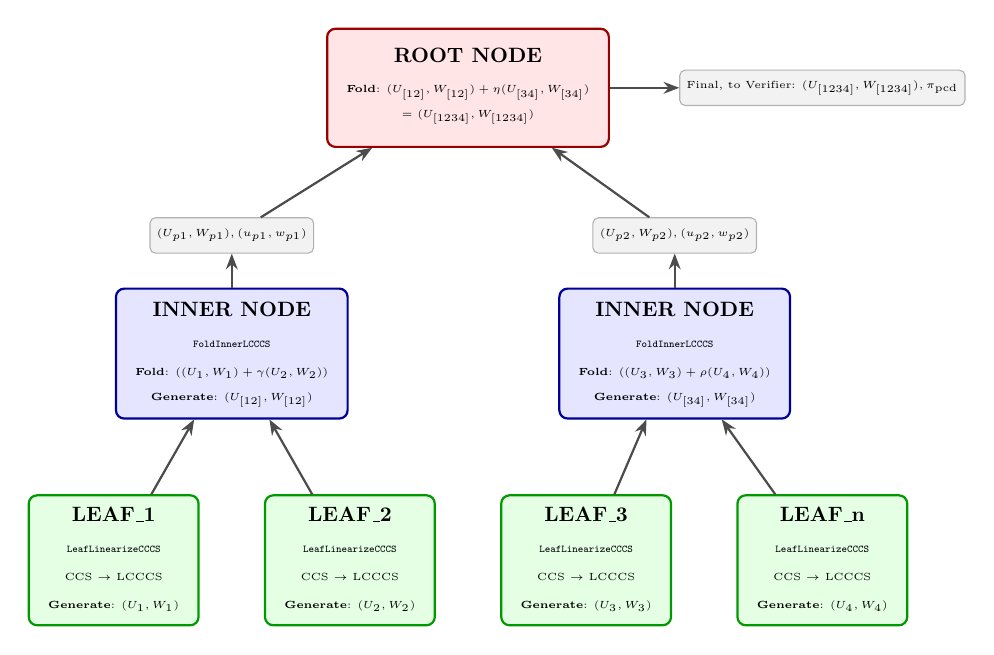
\begin{tikzpicture}[
    scale=0.75,
    every node/.style={transform shape},
    leaf/.style={rectangle, draw=green!60!black, fill=green!10, thick, 
                 minimum width=2.8cm, minimum height=2.2cm, rounded corners=3pt},
    inner/.style={rectangle, draw=blue!60!black, fill=blue!10, thick,
                  minimum width=3.0cm, minimum height=2.2cm, rounded corners=3pt},
    root/.style={rectangle, draw=red!60!black, fill=red!10, thick,
                 minimum width=2.8cm, minimum height=2.0cm, rounded corners=3pt},
    output/.style={rectangle, draw=gray!60, fill=gray!10, 
                   minimum width=2.2cm, minimum height=0.6cm, rounded corners=2pt,
                   font=\tiny},
    arrow/.style={-{Stealth[length=2mm]}, thick, color=black!70}
]

% Root Node (moved up slightly)
\node[root] (root) at (-1.0,8.5) {
    \begin{tabular}{c}
    \textbf{ROOT NODE} \\[0.1cm]
    \tiny \textbf{Fold}: $(U_{[12]}, W_{[12]}) + \eta(U_{[34]}, W_{[34]})$ \\
    \tiny $=$ $(U_{[1234]}, W_{[1234]})$ \\[0.1cm]
    \end{tabular}
};

% Root output (moved further right to avoid overlap)
\node[output] (root_out) at (5.0,8.5) {
    \tiny Final, to Verifier: $(U_{[1234]}, W_{[1234]}), \pi_{\text{pcd}}$
};

% Inner outputs (moved down to give more space for arrows to root)
\node[output] (inner1_out) at (-5.0,6.0) {
    \tiny $(U_{p1}, W_{p1}), (u_{p1}, w_{p1})$
};

\node[output] (inner2_out) at (2.5,6.0) {
    \tiny $(U_{p2}, W_{p2}), (u_{p2}, w_{p2})$
};

% Inner Nodes
\node[inner] (inner1) at (-5.0,4.0) {
    \begin{tabular}{c}
    \textbf{INNER NODE} \\[0.1cm]
    \tiny \texttt{FoldInnerLCCCS} \\[0.05cm]
    \tiny \textbf{Fold}: $((U_{1}, W_{1})+ \gamma(U_{2}, W_{2}))$ \\
    \tiny \textbf{Generate}: $(U_{[12]}, W_{[12]})$
    \end{tabular}
};

\node[inner] (inner2) at (2.5,4.0) {
    \begin{tabular}{c}
    \textbf{INNER NODE} \\[0.1cm]
    \tiny \texttt{FoldInnerLCCCS} \\[0.05cm]
    \tiny \textbf{Fold}: $((U_{3}, W_{3})+ \rho(U_{4}, W_{4}))$ \\
    \tiny \textbf{Generate}: $(U_{[34]}, W_{[34]})$
    \end{tabular}
};

% Leaf Nodes
\node[leaf] (leaf1) at (-7.0,0.5) {
    \begin{tabular}{c}
    \textbf{LEAF\_1} \\[0.1cm]
    \tiny \texttt{LeafLinearizeCCCS} \\[0.05cm]
    \tiny CCS $\rightarrow$ LCCCS \\[0.05cm]
    \tiny \textbf{Generate}: $(U_1, W_1)$
    \end{tabular}
};

\node[leaf] (leaf2) at (-3.0,0.5) {
    \begin{tabular}{c}
    \textbf{LEAF\_2} \\[0.1cm]
    \tiny \texttt{LeafLinearizeCCCS} \\[0.05cm]
    \tiny CCS $\rightarrow$ LCCCS \\[0.05cm]
    \tiny \textbf{Generate}: $(U_2, W_2)$
    \end{tabular}
};

\node[leaf] (leaf3) at (1.0,0.5) {
    \begin{tabular}{c}
    \textbf{LEAF\_3} \\[0.1cm]
    \tiny \texttt{LeafLinearizeCCCS} \\[0.05cm]
    \tiny CCS $\rightarrow$ LCCCS \\[0.05cm]
    \tiny \textbf{Generate}: $(U_3, W_3)$
    \end{tabular}
};

\node[leaf] (leaf4) at (5.0,0.5) {
    \begin{tabular}{c}
    \textbf{LEAF\_n} \\[0.1cm]
    \tiny \texttt{LeafLinearizeCCCS} \\[0.05cm]
    \tiny CCS $\rightarrow$ LCCCS \\[0.05cm]
    \tiny \textbf{Generate}: $(U_4, W_4)$
    \end{tabular}
};

% Arrows showing data flow
\draw[arrow] (leaf1) -- (inner1);
\draw[arrow] (leaf2) -- (inner1);
\draw[arrow] (leaf3) -- (inner2);
\draw[arrow] (leaf4) -- (inner2);
\draw[arrow] (inner1.north) -- (inner1_out.south);
\draw[arrow] (inner2.north) -- (inner2_out.south);
\draw[arrow] (inner1_out) -- (root);
\draw[arrow] (inner2_out) -- (root);
\draw[arrow] (root.east) -- (root_out.west);

\end{tikzpicture}
\caption{HyperNova Tree structure showing leaf linearization and inner node folding}
\end{figure}

\subsection{Two-Layer Commitment Structure}

TreeFold employs different commitment schemes at different levels for optimal efficiency:

\subsubsection{Layer 1: Witness Commitments (Pedersen)}

Each leaf $j$ commits to its witness using Pedersen:
\begin{equation}
C_j = \text{Pedersen}_{\Com}(w_j; r_j)
\end{equation}

These commitments support the homomorphic operations required for folding:
\begin{equation}
C_{\text{fold}} = \rho \cdot C_1 + \rho^2 \cdot C_2
\end{equation}

\subsubsection{Layer 2: Tree Aggregation (Poseidon)}

Pedersen commitments are organized into a Merkle tree using Poseidon:
\begin{equation}
h_w = \text{MerkleTree}_{\text{Poseidon}}([C_1, C_2, \ldots, C_T])
\end{equation}

Similarly, public parameters for each leaf are committed:
\begin{equation}
h_{\text{plk}} = \text{MerkleTree}_{\text{Poseidon}}([\text{plk}_1, \text{plk}_2, \ldots, \text{plk}_T])
\end{equation}

This two-layer approach provides:
\begin{itemize}
\item Efficient folding through Pedersen homomorphism
\item Succinct aggregation through Poseidon Merkle trees
\item Constant-size root representation regardless of tree size
\end{itemize}

\subsection{Global Copy Constraints}

Cross-chunk constraints are handled through a permutation argument:

\begin{definition}[Permutation Product]
For chunk $j$ with permutation $\sigma_j$, the partial product is:
\begin{equation}
p_j = \prod_{i \in I_j} \frac{(w_i + \alpha \cdot i) + \beta}{(w_i + \alpha \cdot \sigma_i) + \beta}
\end{equation}
where $(\alpha, \beta)$ are challenges derived via Fiat-Shamir.
\end{definition}

The global constraint is satisfied when:
\begin{equation}
\prod_{j=1}^T p_j = 1
\end{equation}

This product is computed incrementally up the tree:
\begin{itemize}
\item Leaves compute their local $p_j$
\item Inner nodes multiply: $p_{\text{parent}} = p_{\text{left}} \cdot p_{\text{right}}$
\item Root verifies: $p_{\text{root}} = 1$
\end{itemize}

%==============================================================================
\section{Core Algorithms}
%==============================================================================

With TreeFold's architecture established, we now detail the concrete algorithms that transform our theoretical framework into practical computation. These algorithms bridge the gap between architectural design and implementation, showing precisely how instances flow through the tree structure.

The algorithms work in concert to achieve our efficiency goals: leaf linearization prepares instances for tree processing while preserving HyperNova's security guarantees, and inner node folding leverages the multifold algorithm within our tree topology. Together, they deliver the logarithmic complexity that motivates TreeFold's design.

\subsection{Leaf Linearization}

The leaf prover transforms a fresh CCS instance into LCCS format suitable for tree folding.

\begin{algorithm}
\caption{Leaf Linearization}
\begin{algorithmic}[1]
\Require CCS instance $(x, w)$ for operation chunk
\Ensure LCCS instance $U$, augmented circuit proof

\State \textbf{Linearize:} Run HyperNova~\cite{hypernova} sumcheck to convert CCS to LCCS
\State \quad Commit $C \leftarrow \Com(w)$, obtain evaluation point $r_x$, linear values $v_1, \ldots, v_t$
\State \quad Output $U \leftarrow (C, 1, x, r_x, v_1, \ldots, v_t)$

\State \textbf{Tree data:} Compute chunk's contribution to global constraints
\State \quad $p \leftarrow$ permutation product for this chunk's copy constraints
\State \quad $h_w, h_{plk} \leftarrow$ Poseidon hashes of commitment and proving key

\State \textbf{Prove:} Generate augmented circuit proof containing:
\State \quad - Original computation correctness
\State \quad - Sumcheck verification
\State \quad - Tree folding data $(p, h_w, h_{plk})$

\State \Return LCCS instance $U$ and augmented proof
\end{algorithmic}
\end{algorithm}

The augmented circuit at the leaf encodes several constraints:

\begin{enumerate}
\item \textbf{Application Logic}: The original computation (SHA-256, ECDSA, etc.)
\item \textbf{Tree Folding Gadgets}:
   \begin{itemize}
   \item Permutation product computation
   \item Witness commitment and hashing
   \item Parameter commitment and hashing
   \end{itemize}
\item \textbf{Sumcheck Verification}: Ensures the linearization was performed correctly
\end{enumerate}

\begin{figure}[h]
\centering
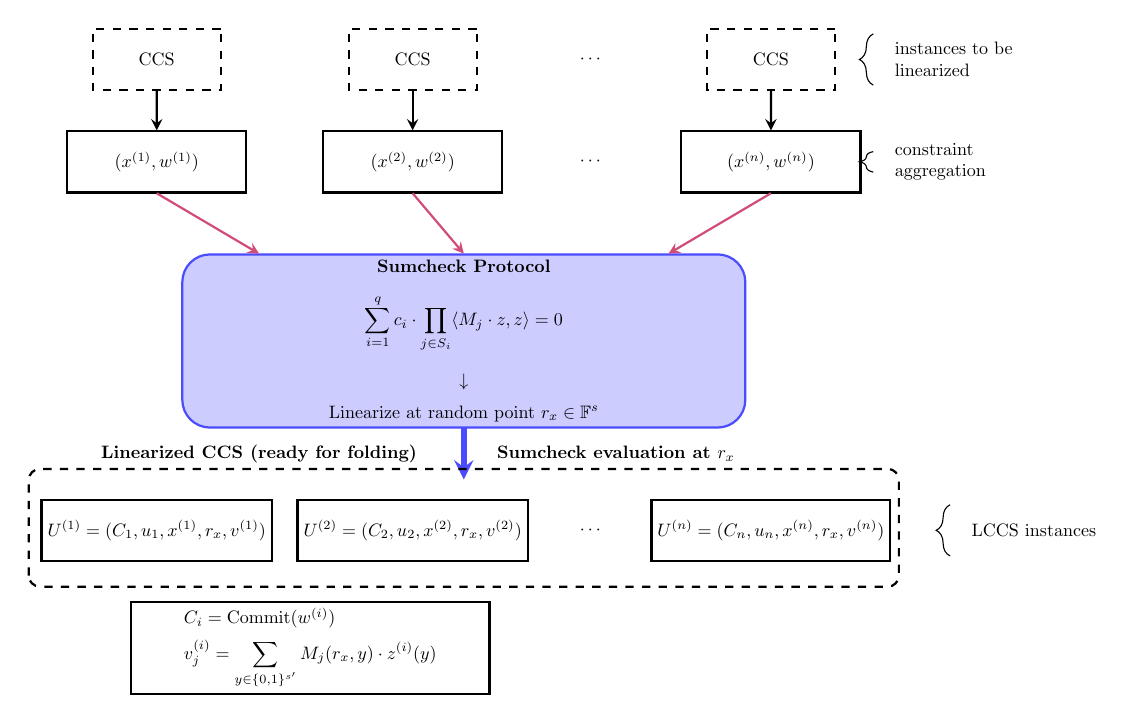
\begin{tikzpicture}[
    scale=0.65,
    transform shape,
    box/.style={rectangle, draw=black, thick, minimum width=3.5cm, minimum height=1.2cm},
    dashedbox/.style={rectangle, draw=black, dashed, thick, minimum width=2.5cm, minimum height=1.2cm},
    bluebox/.style={rectangle, draw=blue!70, fill=blue!20, rounded corners=10pt, thick, minimum width=11cm, minimum height=2.5cm},
    arrow/.style={->, thick, >=stealth},
    purplearrow/.style={->, thick, >=stealth, color=purple!70},
    brace/.style={decorate, decoration={brace, amplitude=5pt, mirror}},
    node distance=1.8cm
]

% Title
% Top row - CCS instances
\node[dashedbox] (ccs1) at (-5, 5) {CCS};
\node[dashedbox] (ccs2) at (0, 5) {CCS};
\node (dots1) at (3.5, 5) {$\cdots$};
\node[dashedbox] (ccsn) at (7, 5) {CCS};

% Brace for instances
\draw[brace] (9, 5.5) -- (9, 4.5) node[midway, right=0.3cm, align=left] {instances to be\\linearized};

% Instance-witness pairs
\node[box] (iw1) at (-5, 3) {$(x^{(1)}, w^{(1)})$};
\node[box] (iw2) at (0, 3) {$(x^{(2)}, w^{(2)})$};
\node (dots2) at (3.5, 3) {$\cdots$};
\node[box] (iwn) at (7, 3) {$(x^{(n)}, w^{(n)})$};

% Arrows from CCS to instance-witness
\draw[arrow] (ccs1) -- (iw1);
\draw[arrow] (ccs2) -- (iw2);
\draw[arrow] (ccsn) -- (iwn);

% Brace for constraint aggregation
\draw[brace] (9, 3.2) -- (9, 2.8) node[midway, right=0.3cm, align=left] {constraint\\aggregation};

% Sumcheck protocol box
\node[bluebox, align=center] (sumcheck) at (1, -0.5) {
    \textbf{Sumcheck Protocol}\\[0.4cm]
    $\displaystyle \sum_{i=1}^q c_i \cdot \prod_{j \in S_i} \langle M_j \cdot z, z \rangle = 0$\\[0.4cm]
    $\downarrow$\\[0.2cm]
    Linearize at random point $r_x \in \mathbb{F}^s$
};

% Purple arrows to sumcheck
\draw[purplearrow] (iw1.south) -- ($(sumcheck.north) + (-4, 0)$);
\draw[purplearrow] (iw2.south) -- ($(sumcheck.north) + (0, 0)$);
\draw[purplearrow] (iwn.south) -- ($(sumcheck.north) + (4, 0)$);

% Arrow pointing down from sumcheck with label - increased spacing
\draw[arrow, blue!70, line width=2pt] (sumcheck.south) -- ++(0, -1.0) node[midway, right=0.5cm, black] {\textbf{Sumcheck evaluation at $r_x$}};

% Dotted box for LCCS instances - moved down
\draw[dashed, thick, rounded corners] (-7.5, -5.3) rectangle (9.5, -3.0);
\node[above] at (-3, -3.0) {\textbf{Linearized CCS (ready for folding)}};

% Bottom row - LCCS instances - moved down
\node[box, minimum width=4.5cm] (lccs1) at (-5, -4.2) {$U^{(1)} = (C_1, u_1, x^{(1)}, r_x, v^{(1)})$};
\node[box, minimum width=4.5cm] (lccs2) at (0, -4.2) {$U^{(2)} = (C_2, u_2, x^{(2)}, r_x, v^{(2)})$};
\node (dots3) at (3.5, -4.2) {$\cdots$};
\node[box, minimum width=4.5cm] (lccsn) at (7, -4.2) {$U^{(n)} = (C_n, u_n, x^{(n)}, r_x, v^{(n)})$};

% LCCS label with brace - adjusted position
\draw[brace] (10.5, -3.7) -- (10.5, -4.7) node[midway, right=0.3cm] {LCCS instances};

% Components explanation box - moved down
\node[box, minimum width=7cm, minimum height=1.5cm, align=left] (components) at (-2, -6.5) {
    $C_i = \text{Commit}(w^{(i)})$\\[0.2cm]
    $v^{(i)}_j = \displaystyle\sum_{y \in \{0,1\}^{s'}} M_j(r_x, y) \cdot z^{(i)}(y)$
};

\end{tikzpicture}
\caption{CCS to LCCS linearization process showing sumcheck transformation}
\end{figure}

\subsection{Inner Node Folding}

Inner nodes fold two LCCS instances from their children into one.

\begin{algorithm}
\caption{Inner Node Folding}
\begin{algorithmic}[1]
\Require Two LCCS instances $U_1, U_2$ from child nodes
\Ensure Folded LCCS instance $U_F$, augmented circuit proof

\State \textbf{Fold:} Run HyperNova folding protocol to combine $U_1, U_2$
\State \quad Derive folding challenge $\rho$, compute linear combination
\State \quad Output $U_F \leftarrow \rho \cdot U_1 + \rho^2 \cdot U_2$

\State \textbf{Tree data:} Aggregate children's contributions to global constraints
\State \quad $p_F \leftarrow p_1 \cdot p_2$ (multiply permutation products)
\State \quad $h_w, h_{plk} \leftarrow$ Poseidon aggregation of child hashes

\State \textbf{Prove:} Generate augmented circuit proof containing:
\State \quad - Folding correctness verification
\State \quad - Tree constraint aggregation
\State \quad - Hash tree updates

\State \Return Folded LCCS instance $U_F$ and augmented proof
\end{algorithmic}
\end{algorithm}

\subsection{Augmented Circuits Design}

TreeFold employs three specialized circuits:

\subsubsection{$\pi_{\text{lin}}$: Leaf Linearization Circuit}

Circuit $F^{\text{lin}}_{\alpha,\beta}(x, w, r_x, v_1, \ldots, v_t, p, h_w, h_{plk})$ verifies CCS-to-LCCS transformation. The circuit enforces the following constraints:

\begin{tcolorbox}[title=Leaf Linearization Circuit Constraints]
\begin{enumerate}[itemsep=5pt]
\item \textbf{Original CCS constraints:} 
\begin{equation}
\sum_{i=1}^q c_i \prod_{j \in S_i} \langle M_j z, z \rangle = 0
\end{equation}

\item \textbf{Linearization correctness:} For all $j \in [t]$:
\begin{equation}
v_j = \sum_{y \in \{0,1\}^{s'}} M_j(r_x, y) z(y)
\end{equation}

\item \textbf{Commitment hash integrity:}
\begin{equation}
h_w = \text{Poseidon}(\Com(w))
\end{equation}

\item \textbf{Proving key hash integrity:}
\begin{equation}
h_{plk} = \text{Poseidon}(\text{pk})
\end{equation}

\item \textbf{Permutation product computation:}
\begin{equation}
p = \prod_{i \in \text{chunk}} \frac{w_i + \alpha \cdot i + \beta}{w_i + \alpha \cdot \sigma(i) + \beta}
\end{equation}
\end{enumerate}
\end{tcolorbox}


\subsubsection{$\pi_{\text{pcd}}$: Inner Node Folding Circuit}

Circuit $F^{\text{pcd}}_{\rho}(U_1, U_2, p_1, p_2, h_{w,1}, h_{w,2}, h_{plk,1}, h_{plk,2})$ verifies correct folding of child instances. The circuit enforces:

\begin{tcolorbox}[title=Inner Node Folding Circuit Constraints]
\begin{enumerate}[itemsep=5pt]
\item \textbf{Instance folding:}
\begin{equation}
U_F = \rho \cdot U_1 + \rho^2 \cdot U_2
\end{equation}

\item \textbf{Permutation product aggregation:}
\begin{equation}
p_F = p_1 \cdot p_2
\end{equation}

\item \textbf{Witness hash aggregation:}
\begin{equation}
h_{w,F} = \text{Poseidon}(h_{w,1} \| h_{w,2})
\end{equation}

\item \textbf{Parameter hash aggregation:}
\begin{equation}
h_{plk,F} = \text{Poseidon}(h_{plk,1} \| h_{plk,2})
\end{equation}

\item \textbf{Commitment folding:}
\begin{equation}
C_F = \rho \cdot C_1 + \rho^2 \cdot C_2
\end{equation}
\end{enumerate}
\end{tcolorbox}

\subsubsection{$C_{EC}$: Elliptic Curve Circuit}

Circuit $F^{\text{EC}}_{\rho}(C_1, C_2 \in \G_1, \rho)$ handles elliptic curve arithmetic in the base field. This circuit is necessary because the main circuit operates over a different field than the commitment curve.

\begin{tcolorbox}[title=Elliptic Curve Circuit Constraints]
\begin{enumerate}[itemsep=5pt]
\item \textbf{Elliptic curve addition:}
\begin{equation}
C_{\text{out}} = \rho \cdot C_1 + \rho^2 \cdot C_2
\end{equation}

\item \textbf{Group membership:}
\begin{equation}
C_1, C_2, C_{\text{out}} \in \G_1
\end{equation}

\item \textbf{Implementation note:} 
When the main circuit uses BN254, this circuit operates over Grumpkin to form a 2-cycle~\cite{cyclefold}.
\end{enumerate}
\end{tcolorbox}


%==============================================================================
\section{Security Analysis}
%==============================================================================

Having detailed TreeFold's implementation through concrete algorithms, we now establish the security guarantees that ensure our efficiency gains do not compromise cryptographic soundness. The transition from sequential to tree-structured folding must preserve the essential security properties that make HyperNova trustworthy.

We establish three fundamental security properties for TreeFold: folding correctness ensures that tree operations preserve statement validity, perfect completeness guarantees that honest provers always succeed, and knowledge soundness prevents malicious provers from creating false proofs. These properties collectively ensure that TreeFold's logarithmic efficiency comes without security trade-offs.

\subsection{Folding Correctness}

The folding operation must preserve the validity of the underlying statements.

\begin{theorem}[Folding Correctness]
Given valid instances $(X_1, W_1), (X_2, W_2) \in R_{\text{LCCS}}$ and folding challenge $\rho$, the folded instance $(X_F, W_F)$ computed by TreeFold satisfies $(X_F, W_F) \in R_{\text{LCCS}}$.
\end{theorem}

\begin{proof}[Proof Sketch]
The proof proceeds by checking each component:

\textbf{Commitment Correctness}: By Pedersen homomorphism:
\begin{equation}
\Com(W_F) = \Com(\rho W_1 + \rho^2 W_2) = \rho \Com(W_1) + \rho^2 \Com(W_2) = C_F
\end{equation}

\textbf{Linear Constraints}: For linear values $v_j$:
\begin{equation}
v_{j,F} = \langle a_j, W_F \rangle = \langle a_j, \rho W_1 + \rho^2 W_2 \rangle = \rho v_{j,1} + \rho^2 v_{j,2}
\end{equation}

\textbf{Non-linear Aggregation}: Permutation products multiply correctly since chunks have disjoint domains. Merkle hashes aggregate via Poseidon maintaining tree structure.
\end{proof}

\subsection{Perfect Completeness}

Valid computations must always produce accepting proofs.

\begin{theorem}[Perfect Completeness]
For every valid witness $(w_1, \ldots, w_n)$ satisfying the computation, TreeFold produces a proof that the verifier accepts with probability 1.
\end{theorem}

The key insight is that validity propagates from leaves to root:
\begin{itemize}
\item Leaves: CCS constraints satisfied $\Rightarrow$ linearization succeeds
\item Inner nodes: Valid children $\Rightarrow$ folding produces valid parent
\item Root: Permutation product equals 1, Merkle roots match commitments
\end{itemize}

\subsection{Knowledge Soundness}

The system must be secure against adversaries attempting to prove false statements.

\begin{theorem}[Knowledge Soundness]
For every PPT adversary $\mathcal{A}$ producing an accepting proof, there exists an efficient extractor $\mathcal{E}$ that outputs a valid witness except with negligible probability.
\end{theorem}

The extraction works in three layers:
\begin{enumerate}
\item \textbf{PCD Extraction}: Extract the entire proof tree from the root proof
\item \textbf{Folding Extraction}: For each inner node, extract child witnesses
\item \textbf{Leaf Extraction}: Extract original computation witnesses from leaves
\end{enumerate}

Crucially, the folding operation acts as a "knowledge barrier"—producing a valid folding proof requires knowing valid child witnesses, preventing forgeries from propagating up the tree.

%==============================================================================
\section{References}
%==============================================================================

\begin{thebibliography}{9}

\bibitem{hypernova}
Abhiram Kothapalli and Srinath Setty.
\textit{{HyperNova}: Recursive arguments for customizable constraint systems}.
Cryptology {ePrint} Archive, Paper 2023/573, 2023.
\url{https://eprint.iacr.org/2023/573}

\bibitem{kilonova}
Tianyu Zheng, Shang Gao, Yu Guo, and Bin Xiao.
\textit{{KiloNova}: Non-Uniform {PCD} with Zero-Knowledge Property from Generic Folding Schemes}.
Cryptology {ePrint} Archive, Paper 2023/1579, 2023.
\url{https://eprint.iacr.org/2023/1579}

\bibitem{ccs}
Srinath Setty, Justin Thaler, and Riad Wahby.
\textit{Customizable constraint systems for succinct arguments}.
Cryptology {ePrint} Archive, Paper 2023/552, 2023.
\url{https://eprint.iacr.org/2023/552}

\bibitem{mangrove}
Wilson Nguyen, Trisha Datta, Binyi Chen, Nirvan Tyagi, and Dan Boneh.
\textit{Mangrove: A Scalable Framework for Folding-based {SNARKs}}.
Cryptology {ePrint} Archive, Paper 2024/416, 2024.
\url{https://eprint.iacr.org/2024/416}

\bibitem{endgame}
Simon Judd.
\textit{{EndGame}: Field-Agnostic Succinct Blockchain with Arc}.
Cryptology {ePrint} Archive, Paper 2024/1925, 2024.
\url{https://eprint.iacr.org/2024/1925}

\bibitem{cyclefold}
Abhiram Kothapalli and Srinath Setty.
\textit{{CycleFold}: Folding-scheme-based recursive arguments over a cycle of elliptic curves}.
Cryptology {ePrint} Archive, Paper 2023/1192, 2023.
\url{https://eprint.iacr.org/2023/1192}

\bibitem{settyfolding}
Srinath Setty.
\textit{Folding Schemes: Why they matter and how they are not employed in the best way possible}.
HackMD, 2024.
\url{https://hackmd.io/@srinathsetty/folding-schemes}

\end{thebibliography}

\end{document}
